\subsection{Requirement Analysis}
An important mechanism of many applications is allowing users to login using a combination of their username or email, and password. Authentication gives user certain authorization, such as posting recipes and managing them. As was discussed in \ref{sec:owasp-top-10}, features such as access control and authentication is still a prevalent security risk. Secure user authentication and authorization therefore is important for users of CheFeed. The feature development for user authentication and session management includes abilities such as \emph{user registration}, \emph{user login}, \emph{user logout}, and the \emph{authorization} to \emph{create, read, update}, and \emph{delete} recipes.

This section will briefly present the security requirement analysis for user authentication and user management that has been acquired by using SKF. First, a new project is created with SKF as seen in figure \ref{fig:chefeed-project}. This will provide the ability to generate requirements for the created project. Appropriately, the project is named CheFeed.

\begin{figure}
    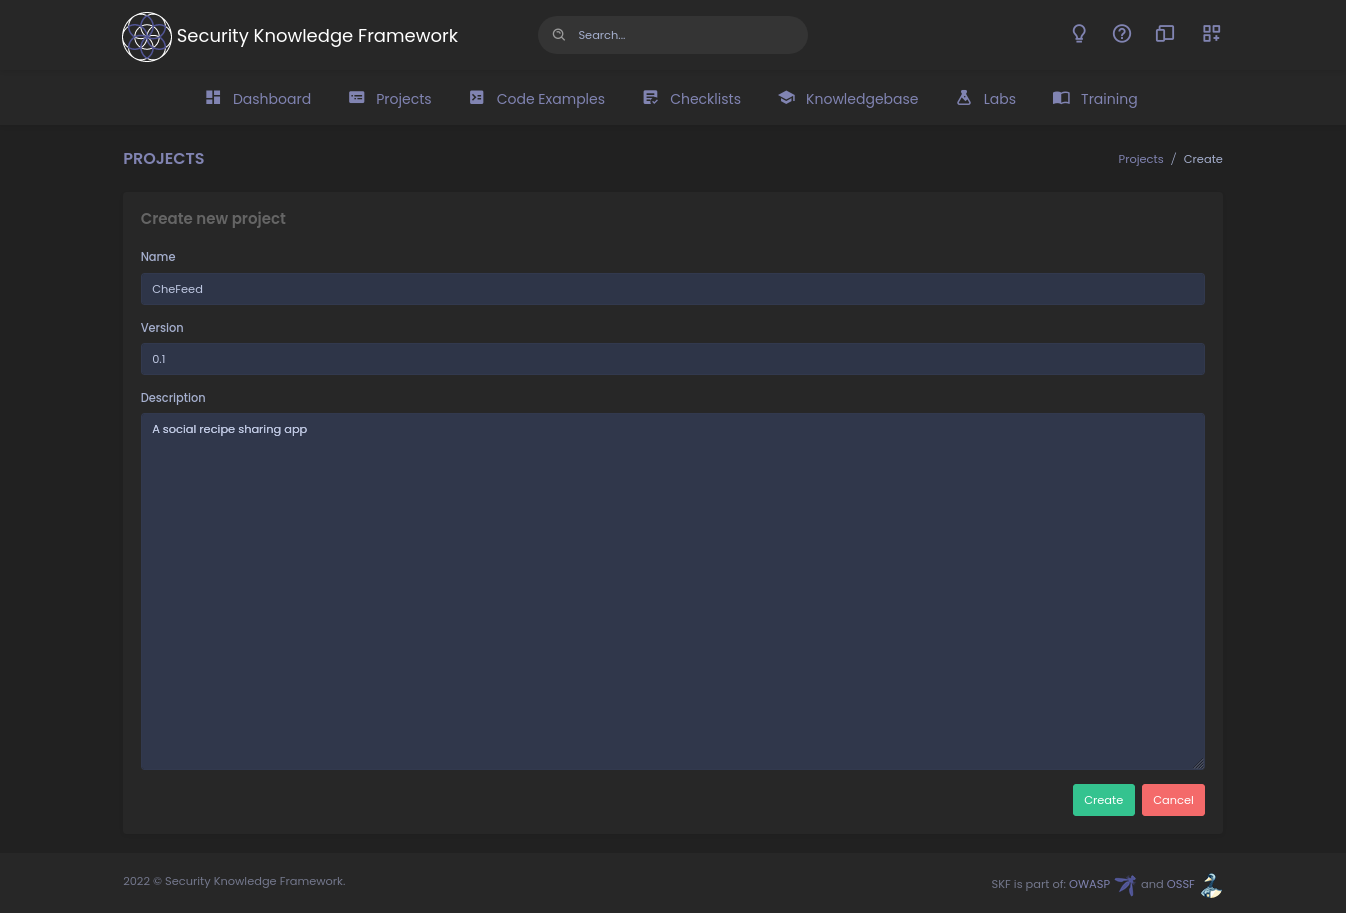
\includegraphics[width=0.5\textwidth]{chapter-4/create-skf-project}
    \caption{Create CheFeed Project}
    \label{fig:chefeed-project}
\end{figure}

\subsubsection{Generating Security Requirements}
The security requirements for user authentication and session management were configured such that it had had the MASVS-L1 security controls in place. The categories considered for its feature development included:
\begin{itemize}
    \item Data Storage and Privacy
    \item Authentication and Session management
\end{itemize}
Figure \ref{fig:skf-checklist-type}, \ref{fig:skf-maturity-level}, \ref{fig:skf-masvs-category}, \ref{fig:skf-sprint-configuration}, \ref{fig:skf-feature-sprint}, and \ref{fig:skf-submit} illustrates the selection process of SKFs security expert system and will be explained briefly.

\paragraph{Checklist Type}
When generating new security requirements for a feature sprint, SKF allows to generate security requirements for either web applications or mobile applications. Additionally, a custom set of requirements can be generated in the dropdown menu. For CheFeed a list of mobile application security requirements are required. Therefore, the mobile application type is selected in this process as seen in figure \ref{fig:skf-checklist-type}. This will generate security requirements based from the MASVS.

\paragraph{Security Maturity Level}
Figure \ref{fig:skf-maturity-level} shows the second step in the security expert wizard is to decide what security maturity level the feature requires, with the options Level 1, Level 2, and Level 3. However, the MASVS does not have a MASVS-L3 maturity level. This seems to be a bug that can be ignored for now. For this study CheFeed implements MASVS-L1, which is recommended for all applications and ensures that it follows the bare minimum.

\paragraph{Categories}
The next step in process is choosing security requirements from the MASVS categories the feature needs as seen. SKF lists out all the MASVS categories and the desired categories can be checked. For the development of CheFeeds user authentication and user session management, requirements from the categories \emph{Data Storage and Privacy} and \emph{Authentication and Session Management} were selected as seen in figure \ref{fig:skf-masvs-category}. The first category provides security controls to protect sensitive data such as user credentials and private information. The second category ensures that that user accounts and sessions are managed securely on the client side, although most of the logic happens at the remote endpoint.

\paragraph{Sprint Configuration}
The sprint configuration step displays a great feature of SKFs security expert system in the requirement analysis phase. This process allows to easily generate the security requirements from the chosen MASVS categories selected in the step before. Based on the answers provided, the correct security requirements will be filtered. Figure \ref{fig:skf-sprint-configuration} shows what configurations were set for CheFeeds user authentication and user sessions feature.

\paragraph{Create Sprint}
Lastly we can create a new feature for the created project or add to an existing one. Since this is a new project with security requirements for a new feature, a new feature is created as seen in figure \ref{fig:skf-feature-sprint}. A name, version and description can be provided to the feature. Lastly, everything can be submitted to generate the security requirements for the feature as seen in figure \ref{fig:skf-submit}.

\begin{figure}
    \centering
    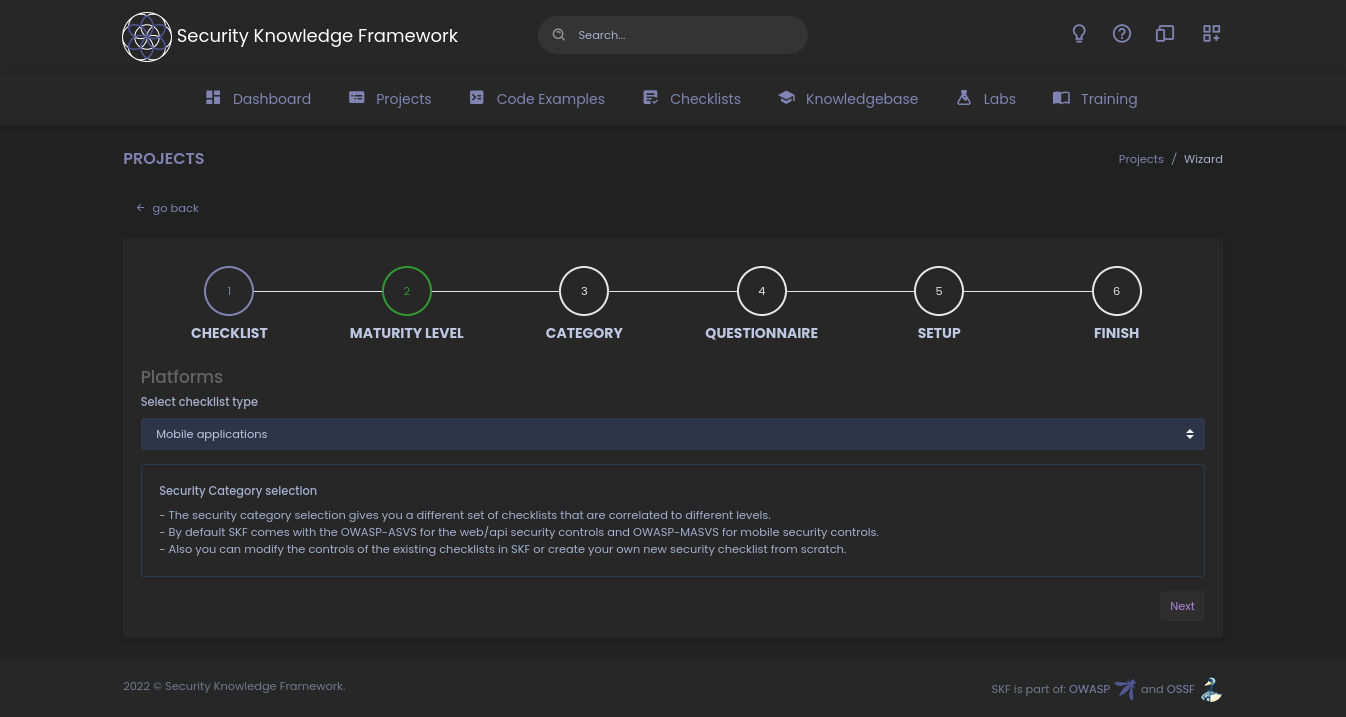
\includegraphics[width=0.5\textwidth]{chapter-4/skf-checklist-type}
    \caption{SKF Security Expert - Select checklist type (security standard)}
    \label{fig:skf-checklist-type}
\end{figure}

\begin{figure}
    \centering
    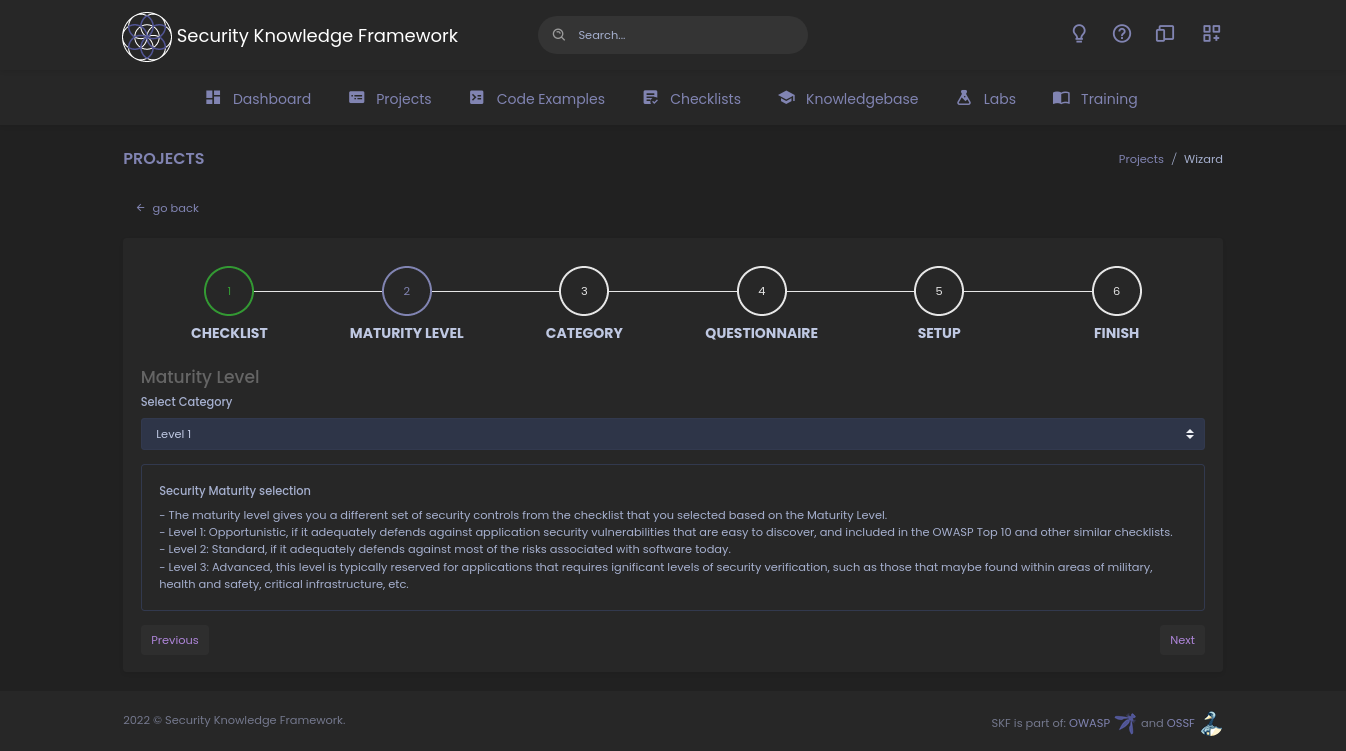
\includegraphics[width=0.5\textwidth]{chapter-4/skf-maturity-level}
    \caption{SKF Security Expert - Select maturity level}
    \label{fig:skf-maturity-level}
\end{figure}

\begin{figure}
    \centering
    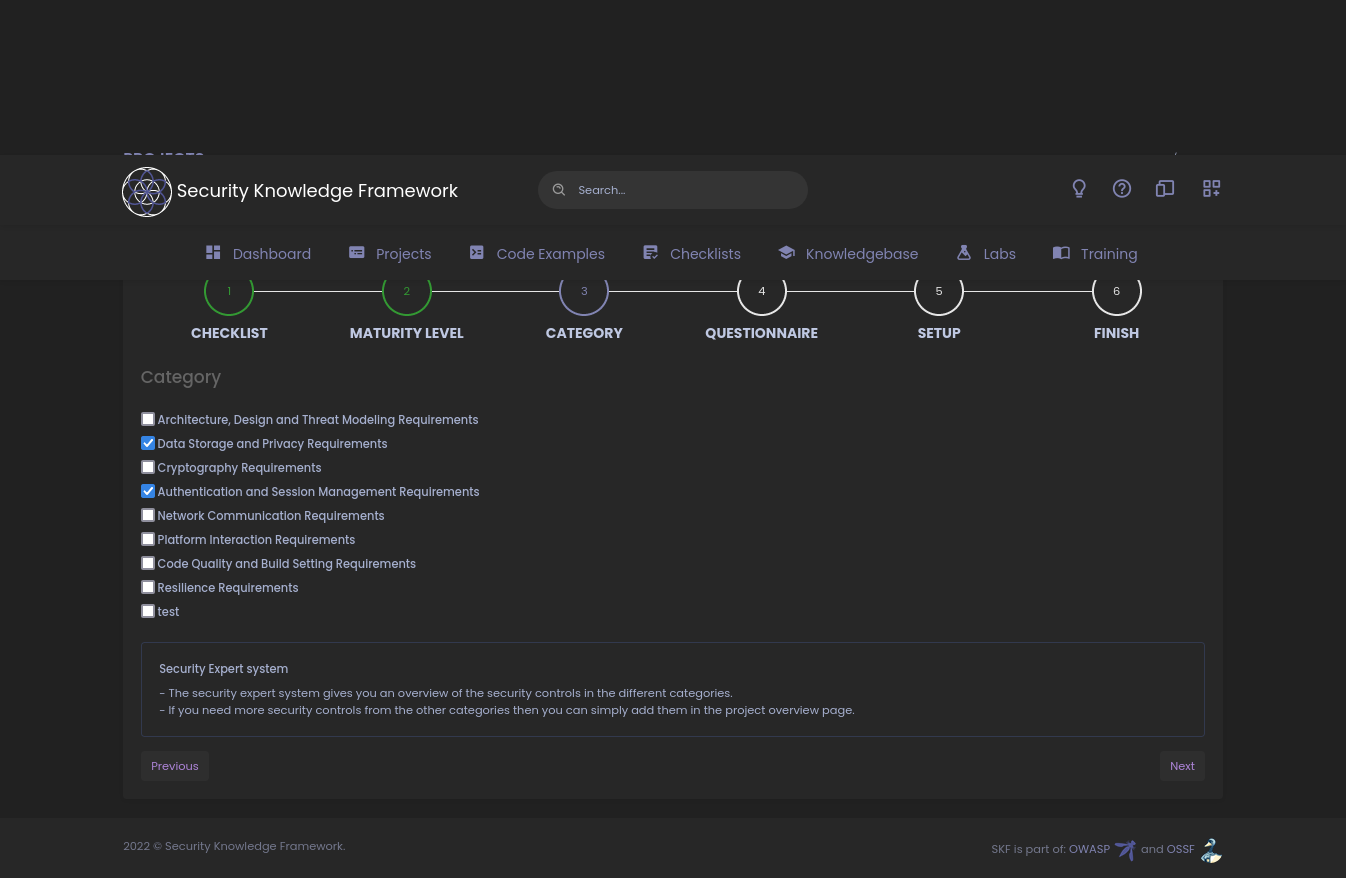
\includegraphics[width=0.5\textwidth]{chapter-4/skf-masvs-category}
    \caption{SKF Security Expert - MASVS Category}
    \label{fig:skf-masvs-category}
\end{figure}

\begin{figure}
    \centering
    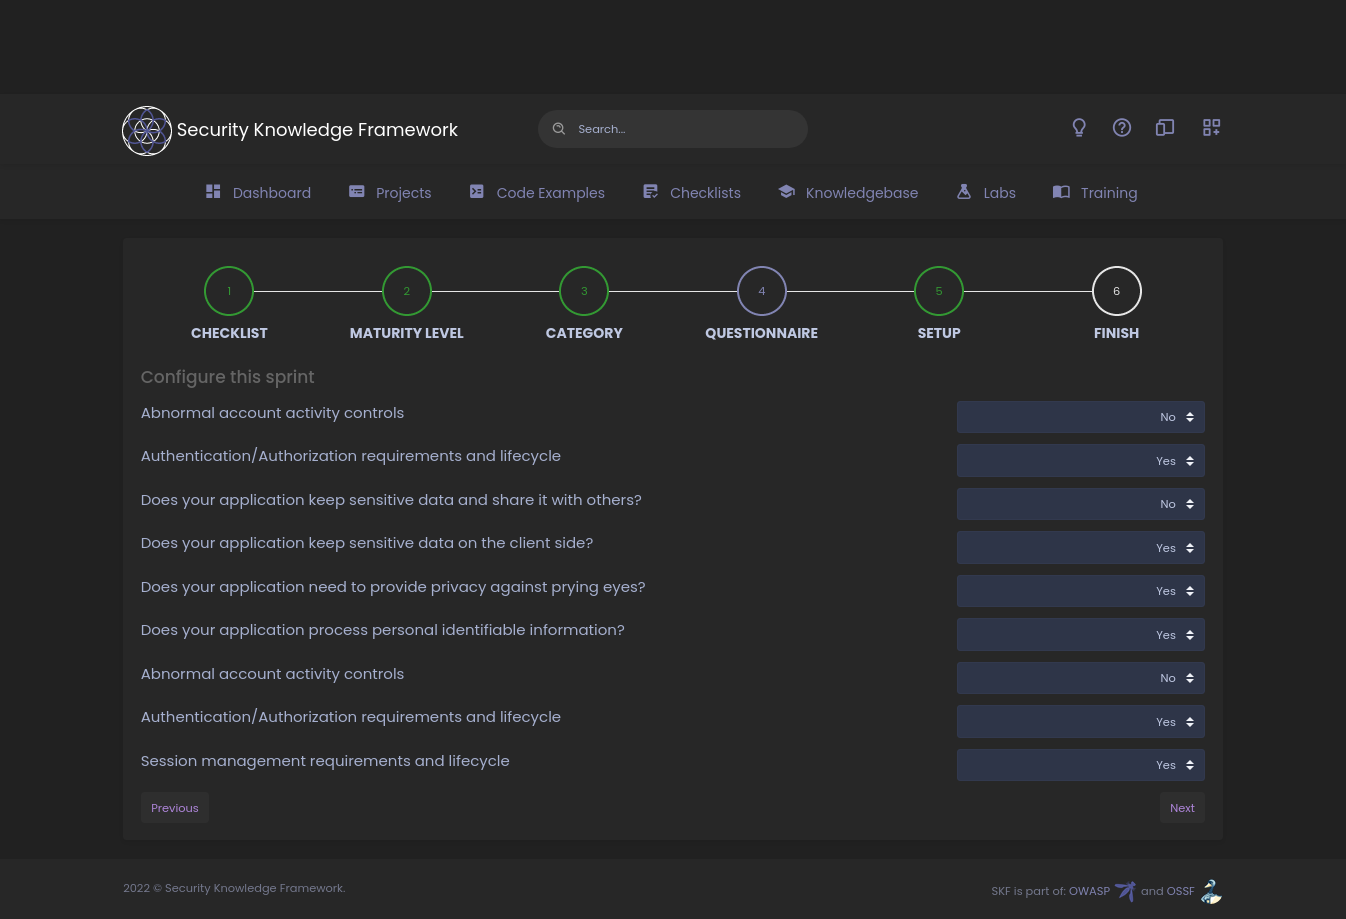
\includegraphics[width=0.5\textwidth]{chapter-4/skf-sprint-configuration}
    \caption{SKF Security Expert - Sprint Configuration}
    \label{fig:skf-sprint-configuration}
\end{figure}

\begin{figure}
    \centering
    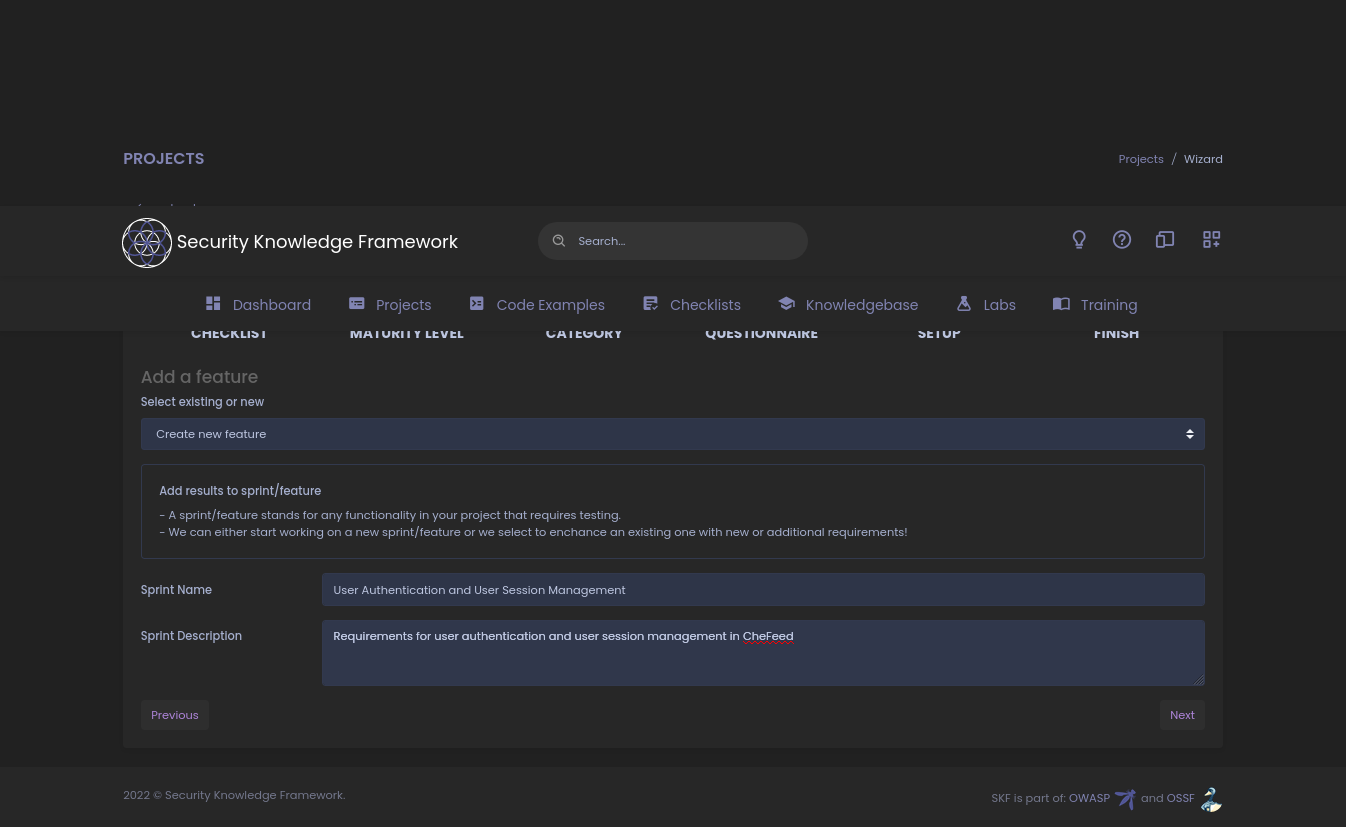
\includegraphics[width=0.5\textwidth]{chapter-4/skf-create-sprint}
    \caption{SKF Security Expert - Create feature sprint}
    \label{fig:skf-feature-sprint}
\end{figure}

\begin{figure}
    \centering
    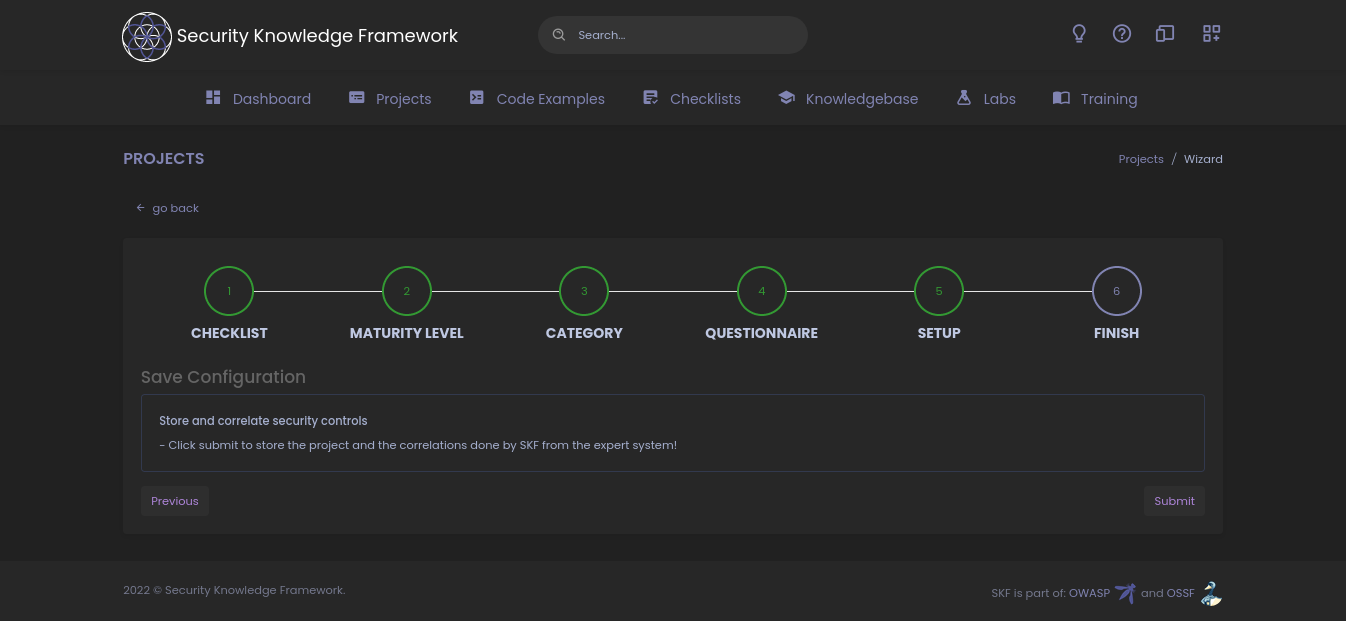
\includegraphics[width=0.5\textwidth]{chapter-4/skf-submit-requirements}
    \caption{SKF Security Expert - Submit}
    \label{fig:skf-submit}
\end{figure}

\paragraph{Requirements Summary}
The process described before generates a summary of security requirements seen in figure \ref{fig:summary-requirements} that can be used further in the design, implementation and testing phase of the SDLC. Table \ref{tab:auth-and-session-summary-requirements} gives a more clear overview of the security requirements summary from figure \ref{fig:summary-requirements}. Fourteen security requirements were gathered in total for the development of user authentication and user session management in CheFeed.

\begin{figure}
    \centering
    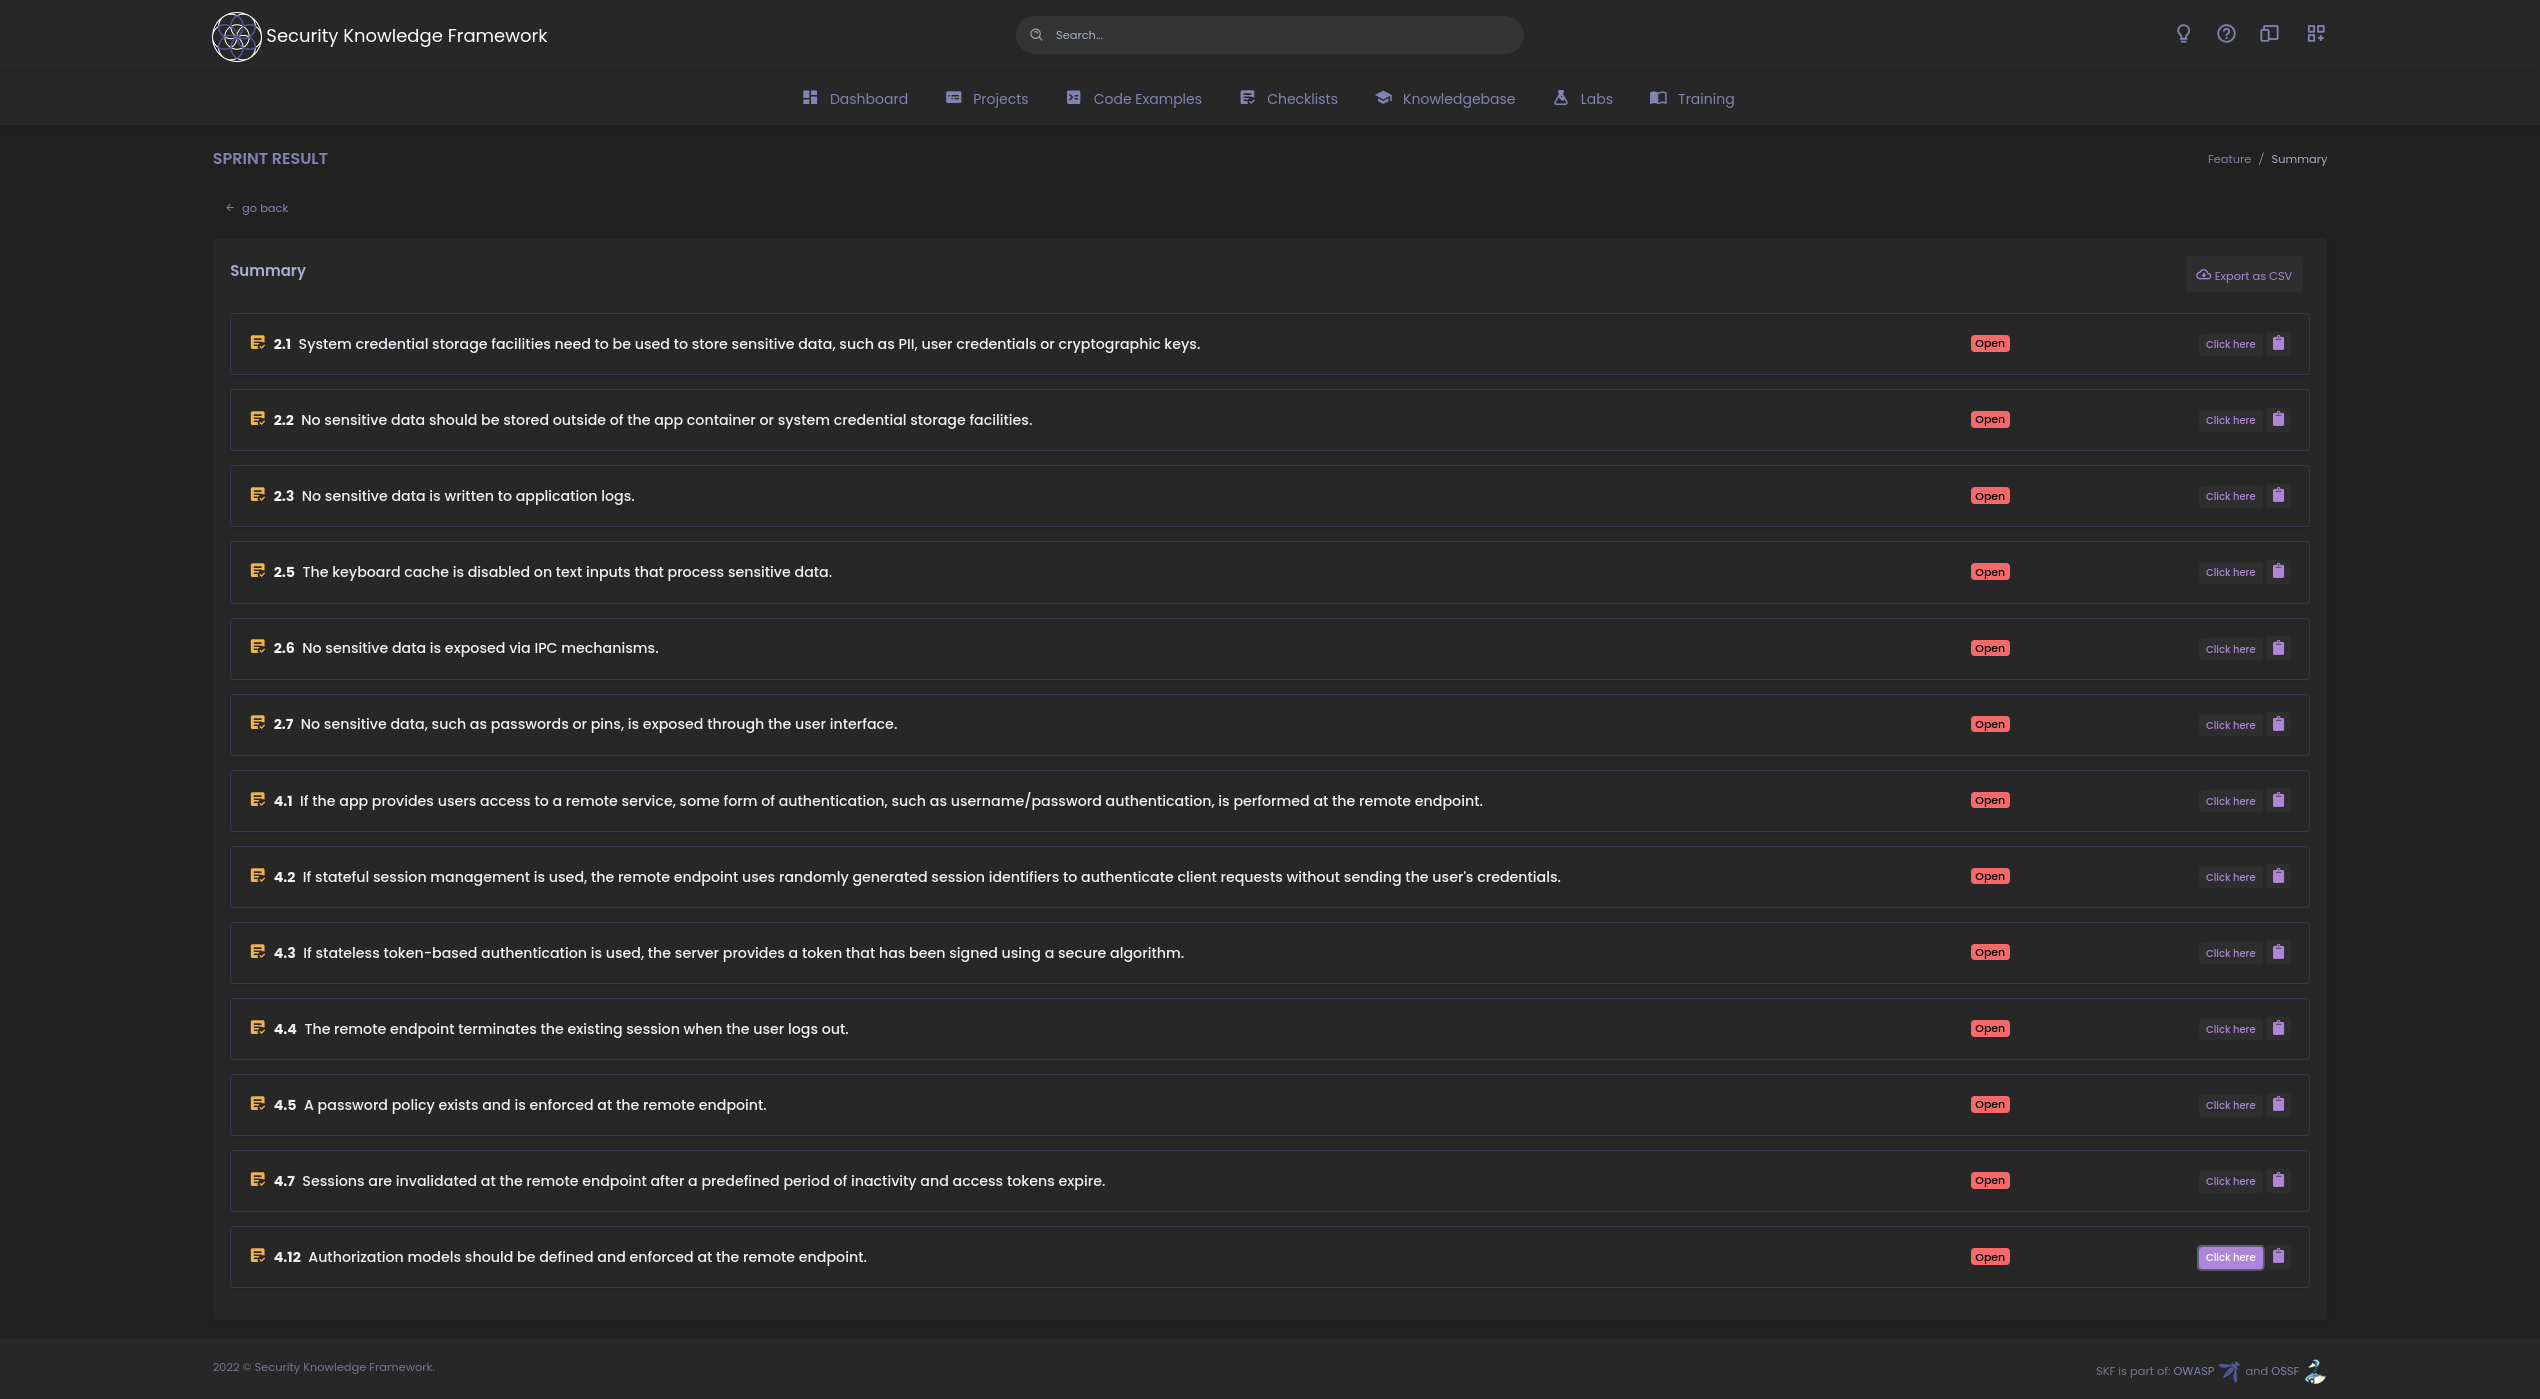
\includegraphics[width=0.5\textwidth]{chapter-4/skf-security-requirements}
    \caption{Summary security requirements}
    \label{fig:summary-requirements}
\end{figure}

\begin{table}
    \centering
    \caption{Summary of user authentication and sessions security requirements}
    \label{tab:auth-and-session-summary-requirements}
    \begin{tabulary}{0.5\textwidth}{|l|L|L|}
        \hline
        \textbf{\#} & \textbf{Category} & \textbf{Description} \\
        \hline
        \textbf{2.1} & Data Storage and Privacy & System credential storage facilities need to be used to store sensitive data, such as PII, user credentials or cryptographic keys \\
        \hline
        \textbf{2.2} & Data Storage and Privacy & No sensitive data should be stored outside of the app container or system credential storage facilities \\
        \hline
        \textbf{2.3} & Data Storage and Privacy & No sensitive data is written to application logs\\
        \hline
        \textbf{2.4} & Data Storage and Privacy & No sensitive data is shared with third parties unless it is a necessary part of the architecture \\
        \hline
        \textbf{2.5} & Data Storage and Privacy & The keyboard cache is disabled on text inputs that process sensitive data \\
        \hline
        \textbf{2.6} & Data Storange and Privacy & No sensitive data is exposed via IPC mechanisms \\
        \hline
        \textbf{2.7} & Data Storage and Pricacy &  No sensitive data, such as passwords or pins, is exposed through the user interface \\
        \hline 
        \textbf{4.1} & Authentication and Session Management & If the app provides users access to a remote service, some form of authentication, such as username/password authentication, is performed at the remote endpoint \\
        \hline
        \textbf{4.2} & Authentication and Session Management & If stateful session management is used, the remote endpoint uses randomly generated session identifiers to authenticate client requests without sending the user's credentials\\
        \hline
        \textbf{4.3} & Authentication and Session Management & If stateless token-based authentication is used, the server provides a token that has been signed using a secure algorithm \\
        \hline
        \textbf{4.4} & Authentication and Session Management & The remote endpoint terminates the existing session when the user logs out \\
        \hline
        \textbf{4.5} & Authentication and Session Management & A password policy exists and is enforced at the remote endpoint \\
        \hline
        \textbf{4.7} & Authentication and Session Management & Sessions are invalidated at the remote endpoint after a predefined period of inactivity and access tokens expire \\
        \hline
        \textbf{4.12} & Authentication and Session Management & Authorization models should be defined and enforced at the remote endpoint \\
        \hline
    \end{tabulary}
\end{table}

\subsection{Design}\label{sec-4:design}
The requirements set the foundation on how the security of the authentication and session management are to be designed. In this section a detailed description of the security design is presented. First, the overall system architecture is presented. Furthemore, user stories are presented that describe the functionality, benefits, and security acceptance criteria to properly mitigate security risks. Lastly a sequence diagram is added to each user story.

\subsubsection{System Architecture}
CheFeed follows a traditional three-tier software architecture as displayed in figure \ref{fig:sys-arch}. The client is the mobile application developed with \textit{react native}. A JavaScript library to develop mobile user interfaces for both Android and iOS devices. It sends and receives requests from the API. The API is developed with FastAPI, a python framework to develop fast APIs. Furthermore, two databases are connected to the API. One to store business data and one to temporarily store random user tokens for user authorization whenever a user starts a new user session. All components for CheFeed are containerized with docker except for the client.

\begin{figure}
    \caption{CheFeed system architecture}
    \label{fig:sys-arch}
    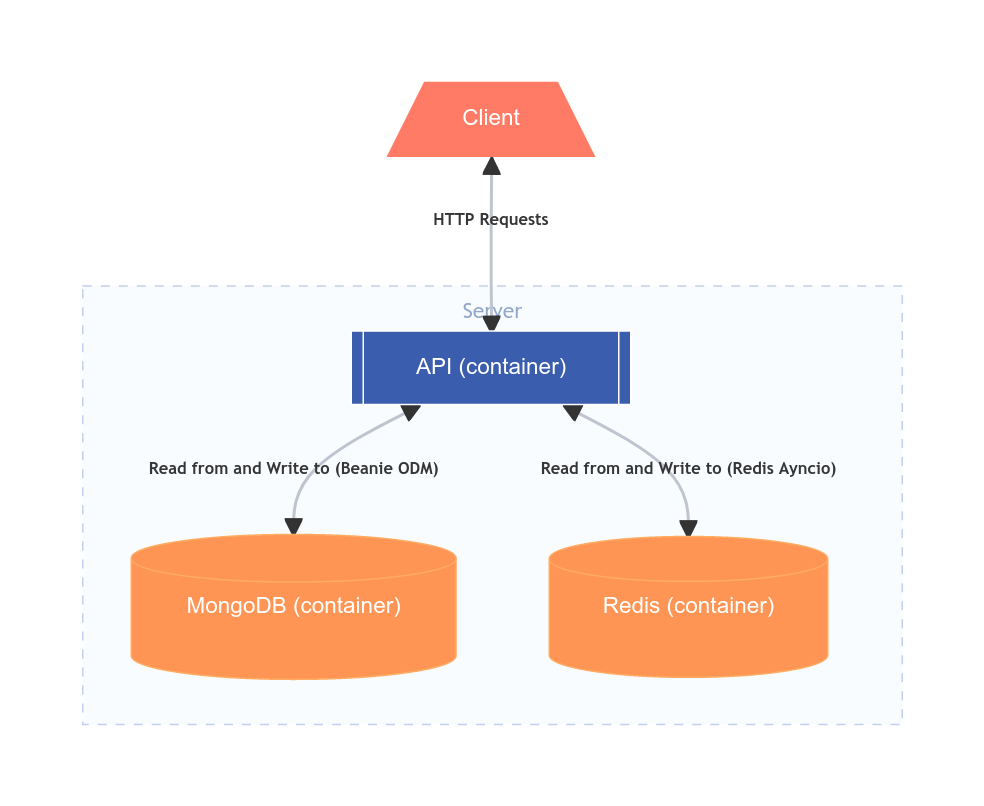
\includegraphics[width=0.5\textwidth]{chapter-4/system-arch}
\end{figure}

\subsubsection{User Stories}
Authentication includes functions such as user registration, login. These are functions that are implemented for CheFeed and have to adhere to the security requirements generated and described in table \ref{tab:auth-and-session-summary-requirements}.

\paragraph{User Registration}
User registration allows users to authenticate themselves in Chefeed using their account. It is the first functionality for the authentication and user sessions feature development. CheFeeds requires users to provide an email address and password to create an account. Table \ref{tab:user-story-register} describes the user story for user registration. 

\begin{table}
    \centering
    \caption{User Story - Register}
    \label{tab:user-story-register}
    \begin{tabulary}{0.5\textwidth}{|l|L|}
        \hline
        \textbf{Description} & As a user I want to be able to register an account for the CheFeed app \\
        \hline
        \textbf{Benefits} & CheFeed hosts user information, including sensitive data. For users to access their stored data, users must be able to authenticate themselves with their registered account. Thus helping ensure that an unauthorized party can access and modify their data \\
        \hline
        \textbf{Acceptance Criteria} &  
        \begin{itemize}
            \item Data storage in source code must be analyzed
            \item Ensure all possible functionality in the application are triggered in order to ensure data generation
            \item Check all application generated and modified files and ensure that the storage method is sufficiently secure such as SharedPreferences, SQL databases, Realm databases, Internal Storage, External Storage
        \end{itemize} 
        \\
        \hline
    \end{tabulary}
\end{table}

\begin{figure}
    \includegraphics[width=0.5\textwidth]{chapter-4/}
\end{figure}

\paragraph{User Login}
User login allows users to authenticate themselves with their registered account. Table \ref{tab:user-story-login} describes the user story for login and figure \ref{fig:auth-flow} illustrates the authentication flow.

\begin{table}
    \centering
    \caption{User story - Login}
    \label{tab:user-story-login}
    \begin{tabulary}{0.5\textwidth}{|l|L|}
        \hline
        \textbf{Description} & As a registered user I want to be able login into the application \\
        \hline
        \textbf{Benefits} & CheFeed hosts user data, including sensitive information. Each user has their data stored separately, each with their associated account. To access their stored data, users must be able to authenticate themselves securely. \\
        \hline
    \end{tabulary}
\end{table}

\begin{figure}
    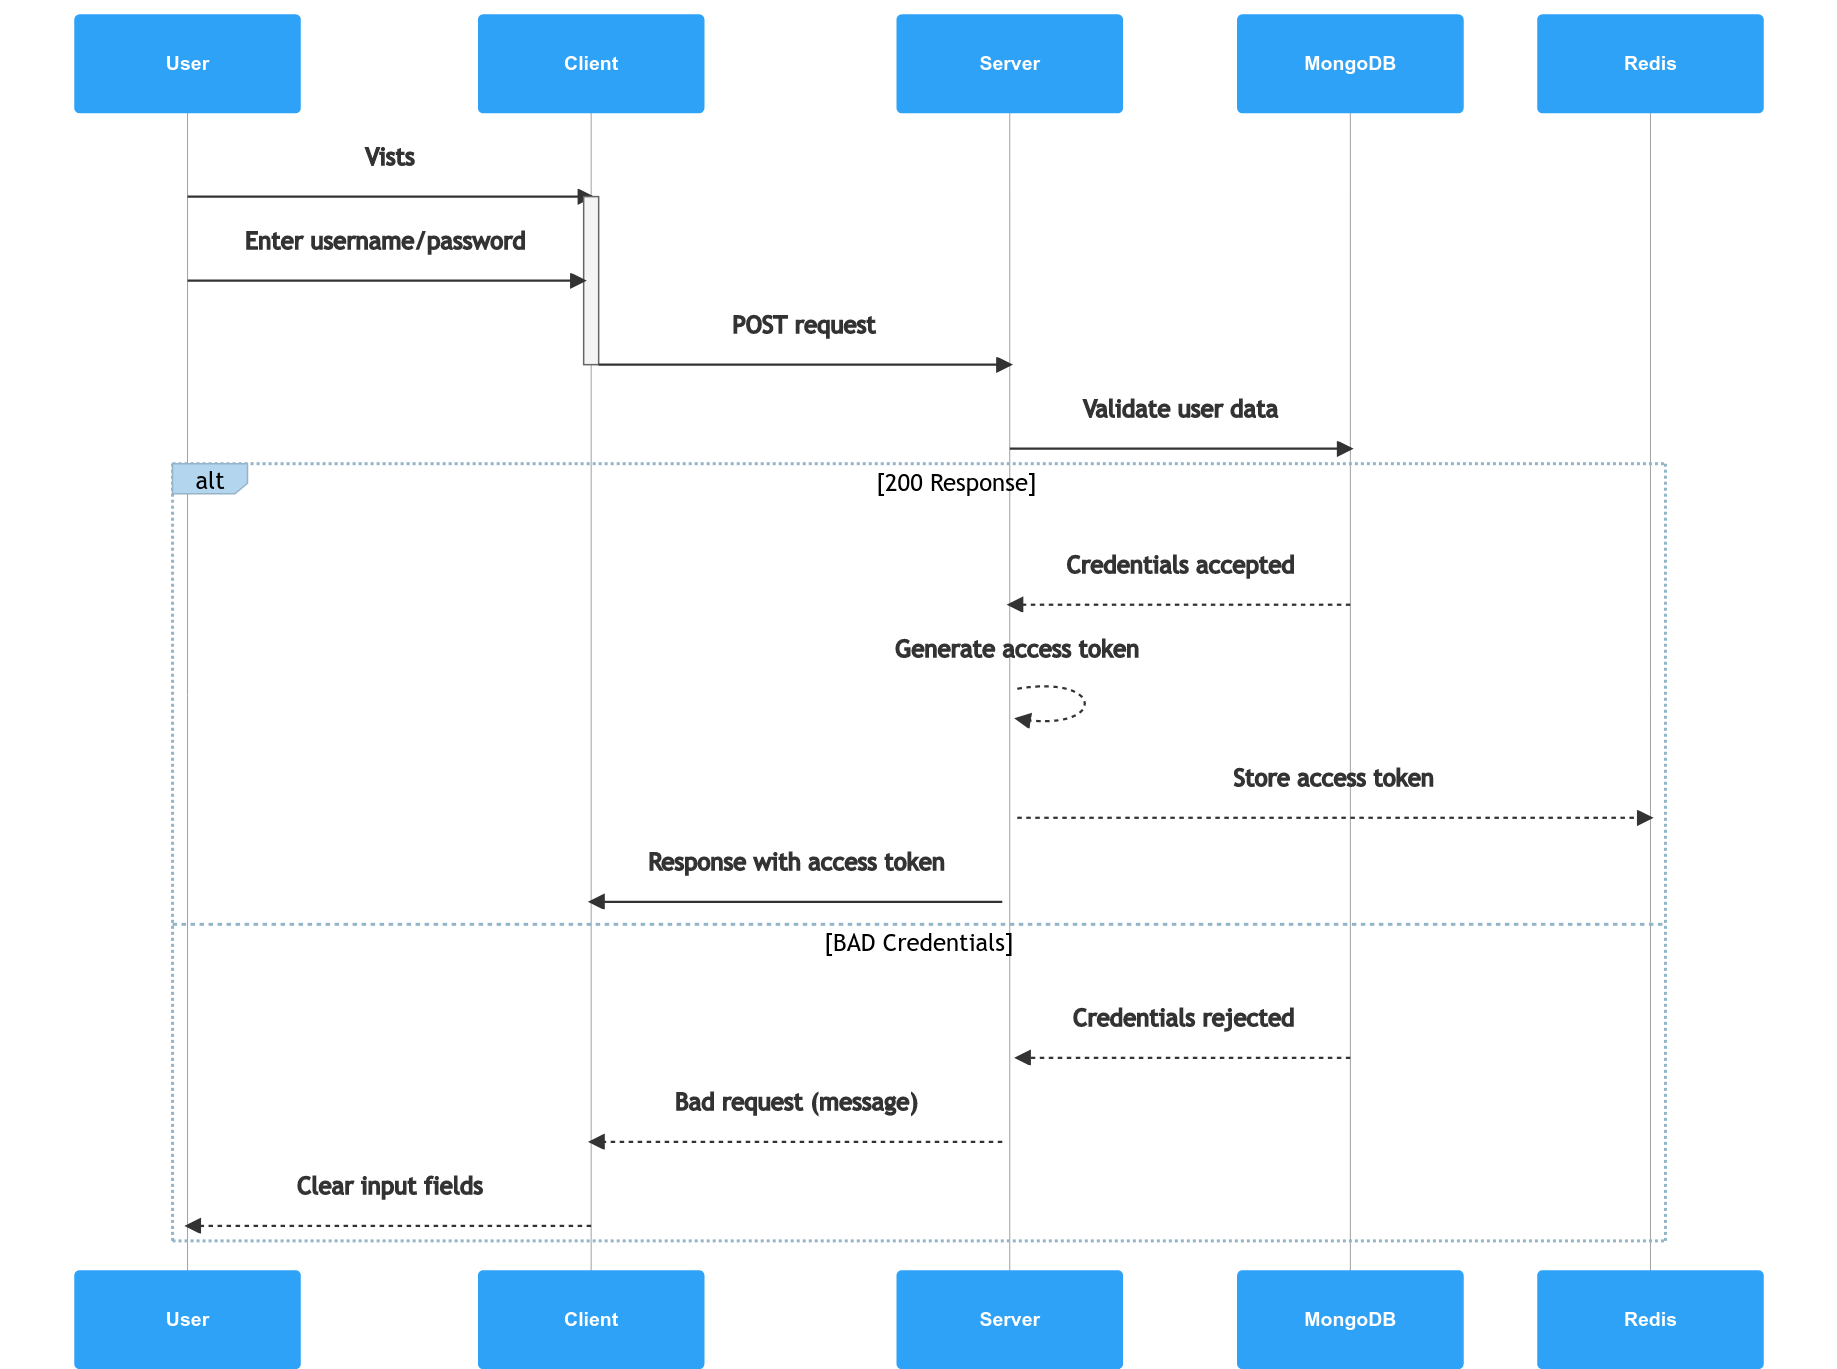
\includegraphics[width=0.5\textwidth]{chapter-4/auth-flow}
    \caption{Authentication flow}
    \label{fig:auth-flow}
\end{figure}
